%%%%%%%%
\section{Contexte : accidents graves des RELs - rétention du corium en cuve}
\Intercalaire{Contexte : stratégie de rétention du corium en cuve pour la mitigation des accidents graves des réacteurs à eau légère}
\subsection{Contexte général des accidents graves des RELs}
\Titre{Contexte général}
\begin{frame}[fragile]
\begin{itemize}
  \item Dans le cadre de l'étude des \emph{``accidents graves''} des réacteurs à eau légère \\ $\rightarrow$ améliorer les moyens de prévention et mitigation associés
  \item Accidents de \emph{fusion du c\oe ur} $\leftarrow$ perte de refroidissement, puissance résiduelle
  \begin{columns}[T]
  \begin{column}{0.7\textwidth}
    \begin{itemize}
      \item \emph{dégradation du c\oe ur} : oxydation exothermique (gaines en Zy), fusion (acier, Zr), dissolution puis fusion (ZrO$_{2-x}$, UO$_2$) \\ $\rightarrow$ \emph{formation d'un bain de ``corium''}
      \item \emph{relocalisation dans le fond de la cuve} \\ $\rightarrow$ interaction corium-eau et risque d'explosion vapeur ; \emph{comportement du corium en fond de cuve}  et risque de perte d'intégrité de la cuve
      \item relocalisation dans le puits de cuve \\ $\rightarrow$ interaction corium-eau  et risque d'explosion vapeur ; étalement, interaction corium-béton et risque de percement du radier
    \end{itemize}
  \end{column}
  \begin{column}{0.25\textwidth}
    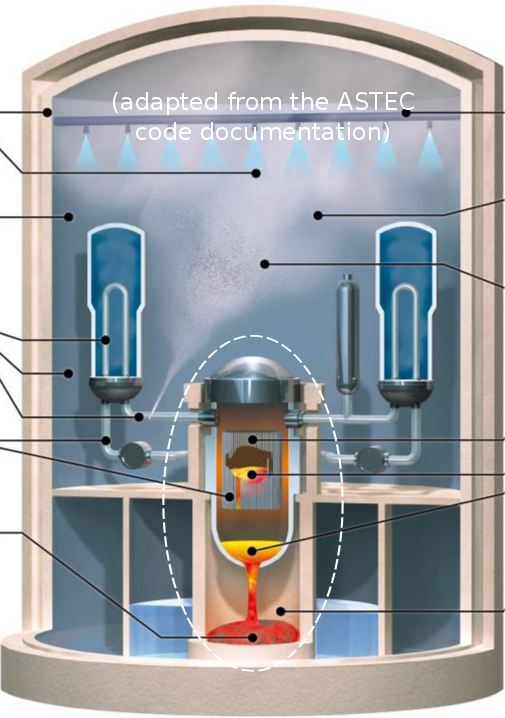
\includegraphics[width=\textwidth]{Figures/corium.png}
  \end{column}
  \end{columns}
  \item \emph{``Physique'' du corium} : ``mal connue'' 
  \begin{itemize}
    \item \emph{phénomènes} nombreux, pas forcément clairement identifiés ou \emph{``mal connus''} 
    \item des \emph{échelles temporelles et spatiales} pouvant très \emph{différentes}
  \end{itemize}
\end{itemize}
\end{frame}
\Titre{Dégradation en c\oe ur et progression de l'accident vers le fond de cuve}
\begin{frame}[fragile]
\begin{center}
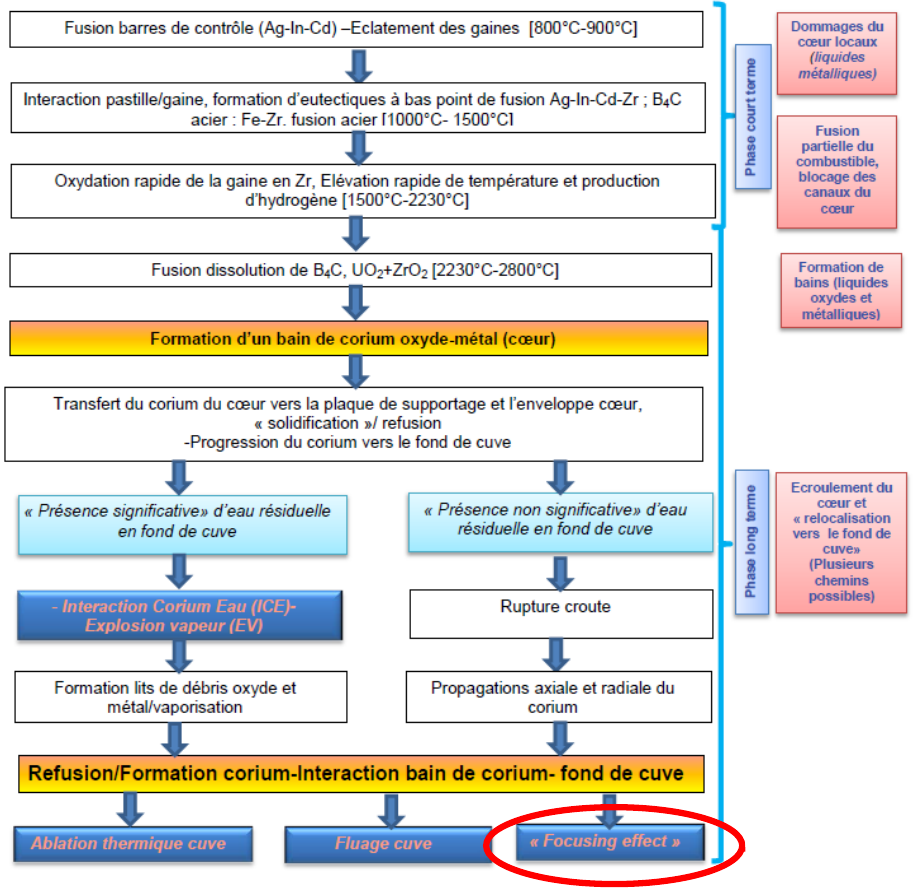
\includegraphics[height=\textheight]{Figures/transition_PP.png}
\end{center}
\end{frame}
\subsection{Ce $\mu$-projet: stratégie de rétention en cuve}
\Titre{Ce $\mu$-projet: stratégie de rétention en cuve}
\begin{frame}[fragile]
Rétention du corium en cuve ou ``In-Vessel Retention'' (IVR)
\begin{columns}
\begin{column}{0.7\textwidth}
\begin{itemize}
\item Quoi~? Une \emph{stratégie de gestion de l'accident de fusion du c\oe ur} introduite dans les années 1990 \cite{Henry1993,Tuomisto1994}
\item Pourquoi~? \emph{Garder l'intégrité de la cuve} pour y contenir les matériaux fondus du c\oe ur
\item Comment~? \emph{Dépressurisation précoce} de la cuve et \emph{renoyage précoce du puits de cuve} 
\end{itemize}
\end{column}
\begin{column}{0.3\textwidth}
\centering 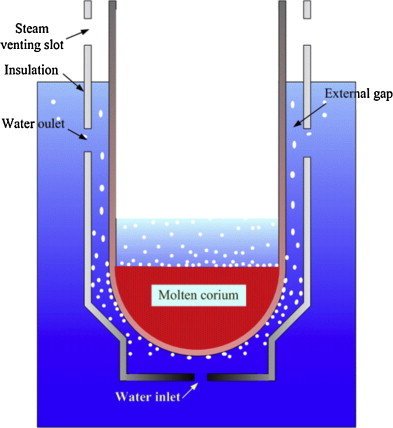
\includegraphics[height=0.5\textheight]{Figures/ivr.jpg}
\end{column}
\end{columns}
\begin{itemize}
\item Une mitigation réussie si :
\begin{itemize}
  \item le \emph{refroidissement de la cuve} par circulation d'eau est ``efficace'' de manière à éviter une ablation (locale) de la cuve sur toute son épaisseur \textit{i.e.} \\
  rester en \emph{régime d'ébullition nucléée} $\leftrightarrow$ éviter la crise d'ébullition (assèchement) $\leftrightarrow$ garantir que le \emph{flux de chaleur} en paroi externe de la cuve reste \emph{inférieur au flux critique}
  \item la cuve, partiellement ablatée, \emph{résiste mécaniquement} à la charge imposée (poids du bain et éventuels pics de pression) en transitoire et sur le long terme
\end{itemize}
\end{itemize}
\end{frame}
\begin{frame}[fragile]
\begin{columns}
\begin{column}{0.45\textwidth}
Trois sujets (interdépendants) pour une démonstration d'IVR:
\begin{itemize}
  \item \emph{comportement du corium en cuve} 
  \item \emph{thermohydraulique diphasique} de l'eau dans le \emph{puits de cuve}
  \item \emph{thermomécanique de la cuve}
\end{itemize}
\end{column}
\begin{column}{0.55\textwidth}
\begin{figure}[H]
\centering 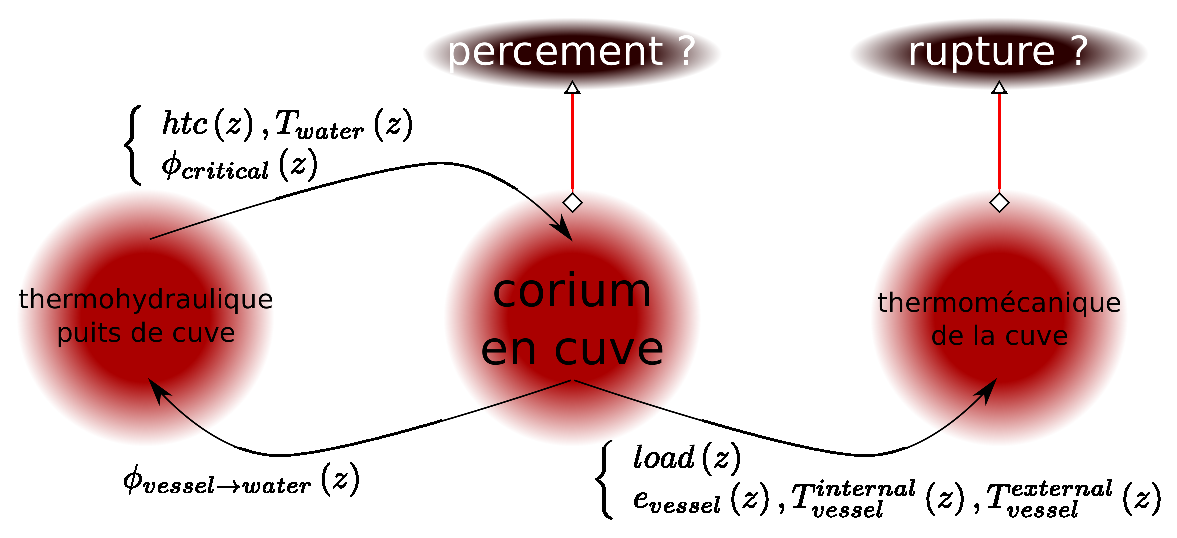
\includegraphics[width=1.0\textwidth]{Figures/ivr_topics.eps}
\caption{Vue schématique des thématiques associées à une démonstration d'IVR}
\end{figure}
\end{column}
\end{columns}
On se concentrera ici sur la question du \emph{comportement du corium en cuve}
\begin{itemize}
\item thermohydraulique multiphasique $\rightarrow$ chargement thermique sur la cuve
\item système ouvert $\leftarrow$ apport d'acier fondu par ablation de structures internes et de la paroi de la cuve
\end{itemize}
\end{frame}

%%%%%%%%
\section{Le corium en fond de cuve: version simple}
\Intercalaire{Le corium en fond de cuve: version simple}
\Titre{Le corium en fond de cuve: version simple}
\begin{frame}[fragile]
Evaluation \emph{stationnaire ``enveloppe''} des flux de chaleur transmis à la cuve
\begin{itemize}
\item approche ``historique'' utilisée en particulier dans la \emph{démonstration de sûreté} des réacteurs AP600 puis \emph{AP1000} \cite{Esmaili2004} 
\item dans sa version initiale, \emph{configuration ``à deux couches''} :
\begin{columns}[T]
    \begin{column}{0.35\textwidth}
      \begin{figure}[H]
\centering 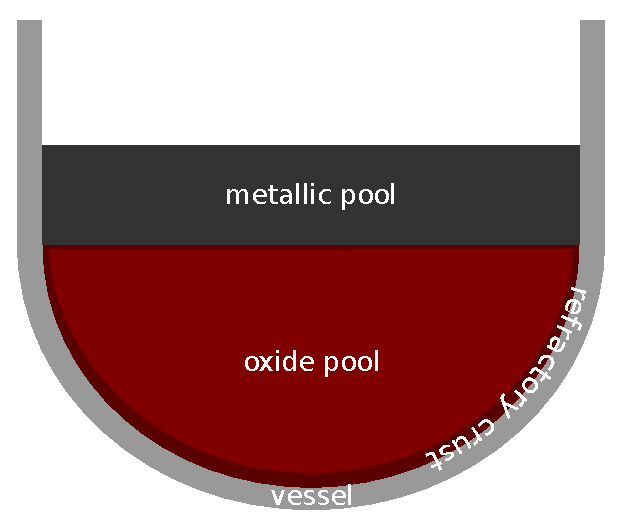
\includegraphics[height=0.4\textheight]{Figures/TD_2layer_2.eps}
\caption{Configuration à deux couches}
      \end{figure}
    \end{column}
    \begin{column}{0.65\textwidth}
    \begin{itemize}
    \item en bas : une \emph{phase oxyde} entourée d'une croûte réfractaire 
    \item en haut : une \emph{phase métallique} en contact direct avec la paroi de la cuve en fusion
    \item masses et compositions de ces deux couches obtenus à partir de simulations de la dégradation en c\oe ur et d'hypothèses simplistes sur la fusion des structures et de la paroi de la cuve
    \end{itemize}
    \end{column}
\end{columns}
  \item utilisée pour des \emph{études statistiques avec une modélisation intégrale} (\textit{cf.} TD à venir) : paramètres du modèle et définissant la configuration en fond de cuve ``probabilisés'' 
\end{itemize}

\end{frame}
\Titre{Corium en cuve et écoulements en convection naturelle}
\begin{frame}[fragile]
Deux configurations d'\emph{écoulements en convection naturelle} :
\begin{columns}[T]
    \begin{column}{0.3\textwidth}
\centering 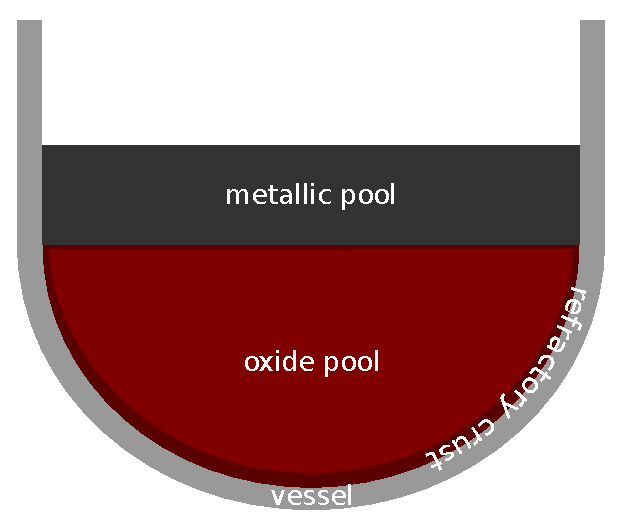
\includegraphics[height=0.3\textheight]{Figures/TD_2layer_2.eps}
    \end{column}
    \begin{column}{0.7\textwidth}
    \begin{itemize}
    \item couche métallique supérieure chauffée par le dessous, refroidie latéralement, par le dessus
    \item bain oxyde chauffé ``en volume'' et refroidie à sa frontière
    \end{itemize}
    \end{column}
\end{columns}
\vskip \baselineskip
\emph{Propriétés des liquides mis en jeu} et comparison à l'eau liquide 
\begin{tiny} \begin{center}
  \begin{tabularx}{0.9\textwidth}{|l|R|R|R|R|} \hline
  \multicolumn{1}{|c|}{\multirow{2}{*}{Propriété}} & \multicolumn{1}{c|}{\multirow{2}{*}{Unité}} & \multicolumn{2}{c|}{Valeur (\emph{ordre de grandeur})} & Valeur eau \n
  & & \multicolumn{1}{c|}{Oxyde} & \multicolumn{1}{c|}{Métal} & \multicolumn{1}{c|}{à 25$^o$C, 1bar} \n \hline
  masse volumique $\rho$ & kg.m$^{-3}$ & ~8000 & ~7000 & 997 \n
  conductivité thermique $\lambda$ & W.m$^{-1}$.K$^{-1}$ & 5 & 25 & 0.61\n
  \emph{viscosité cinématique} $\nu$ & m$^2$s.$^{-1}$ & 5$\times$10$^{-7}$ & 5$\times$10$^{-7}$ & 8.9$\times$10$^{-7}$ \n
  capacité calorifique massique $Cp$& J.K$^{-1}$.kg$^{-1}$ & 500 & 800 & 4182 \n
  coefficient de dilatation thermique isobare $\beta$ & K$^{-1}$ & 10$^{-4}$ & 10$^{-4}$ & 2.6$\times$10$^{-4}$\n \hline
  diffusivité thermique $\alpha=\frac{\lambda}{\rho Cp}$ & m$^2$s.$^{-1}$ & 10$^{-6}$ & 4$\times$10$^{-6}$ & 1.5$\times$10$^{-7}$ \n
  $\emph{Pr}=\frac{\nu}{\alpha}=\frac{\text{diffusivité de la quantité de mouvement}}{\text{diffusivité de la chaleur}}$ & - & 0.5 & 0.1 & 5.9 \n \hline
  \end{tabularx}
\end{center}
  \begin{remark}
  On considèrera que le corium en cuve peut être traité comme un fluide Newtonien (dans la gamme de température/composition d'intérêt); \danger $\ne$ pour le corium ``hors-cuve''
  \end{remark}
\end{tiny} 
\end{frame}

%%%%%%%%
\subsection{Thermohydraulique de la couche métallique supérieure}
\Titre{Thermohydraulique de la couche métallique supérieure}
\begin{frame}[fragile]
\begin{columns}[T]
    \begin{column}{0.3\textwidth}
\vskip -\baselineskip
\centering 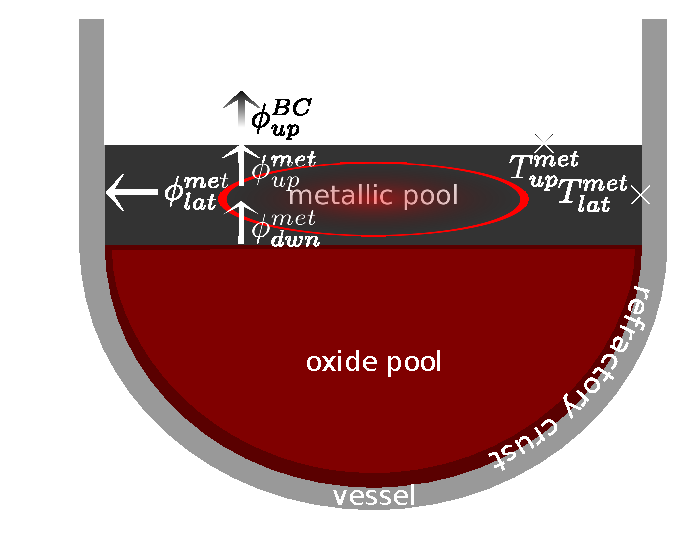
\includegraphics[height=0.4\textheight]{Figures/TD_2layer_metal.eps}
    \end{column}
    \begin{column}{0.7\textwidth}  
    \begin{scriptsize}
    \begin{itemize}
    \item en bas (croûte) : \textit{sans glissement}, $\phi^{met}_{dwn}$ imposé
    \item latéralement (cuve) : {\scriptsize $\left\{\begin{array}{l} \text{sans glissement} \\ T^{met}_{lat} \text{ imposée (fusion) / } \phi^{met}_{lat}=\phi^{vessel}_{lat} \end{array}\right.$}
    \item en haut : {\scriptsize $\left\{\begin{array}{l} \text{sans glissement / surface libre} \\ \text{température imposée} T^{met}_{up} \text{ / } \phi^{met}_{up}=\phi^{met}_{BC} \end{array}\right.$}
    \end{itemize} 
    \end{scriptsize}
    \end{column}
\end{columns}
\begin{itemize}
\item Sous l'\emph{hypothèse de Boussinesq}, équations de conservation locales :
\begin{columns}[T]
    \begin{column}{0.58\textwidth}
\begin{scriptsize}
\vskip -\baselineskip
\begin{eqnarray*}
\div{\vec{v}} &=& 0 \\
\frac{\partial \vec{v}}{\partial t} + \vec{v} \cdot \grad{\vec{v}} &=& -\frac{1}{\rho_0}\grad{p} + \nu_0 \Lapl{\vec{v}} - \vec{g} \beta_0 \left(T-T_0\right) \\
\frac{\partial T}{\partial t} + \vec{v} \cdot \grad{T} &=& \alpha_0 \Lapl{T}
\end{eqnarray*}
\vskip -\baselineskip
\end{scriptsize}
    \end{column}
    \begin{column}{0.42\textwidth}
\begin{scriptsize}
    Bilan thermique intégral :
    \begin{equation*} mCp \frac{d\bar{T}}{dt} = \phi^{met}_{dwn} S^{met}_{dwn} - \phi^{met}_{lat} S^{met}_{lat} - \phi^{met}_{up} S^{met}_{up} \end{equation*}
\end{scriptsize}
    \end{column}
% \vskip -\baselineskip
\end{columns}
\item Les \emph{``paramètres de contrôle''} sont :
\begin{itemize}
\item $Pr$, $Gr=\frac{g\beta\Delta T H^3}{\nu^2}=\frac{\text{forces de gravité}}{\text{forces visqueuses}}$ (ou $Ra=Gr \cdot Pr$)
\item le rapport d'aspect $\frac{H}{R}$ (cylindre de rayon $R$, hauteur $H$)
\item éventuellement d'autres selon les conditions en limite supérieure
\end{itemize}
\item Les `\emph{`quantités d'intérêt''} sont $Nu_{lat}$ et $Nu_{up}$ ($Nu=\frac{\text{flux de chaleur convectif}}{\text{flux de chaleur conductif}}=\frac{htc \times L}{\lambda}$ )
\end{itemize}
\end{frame}
\begin{frame}[fragile]
\begin{itemize}
\item De première importance car possibilité de \emph{concentration de flux (``focusing effect'')} \\ \textit{i.e.} $\frac{\phi^{met}_{lat}}{\phi^{met}_{dwn}}>1$ $\rightarrow$ \emph{risque principal de percement ``thermique'' de la cuve}
\item Configuration étudiée expérimentalement e.g. dans la \emph{campagne BALI-Metal} (CEA Grenoble) : avec de l'eau (\danger $Pr$), en géométrie parallépipédique $\rightarrow$ $\frac{\phi^{met}_{lat}}{\phi^{met}_{dwn}}\left(H\right)$
\item Schéma grossier de l'écoulement (Figure tirée de \cite{Villermaux1999})
\begin{columns}[T]
    \begin{column}{0.6\textwidth}
\centering 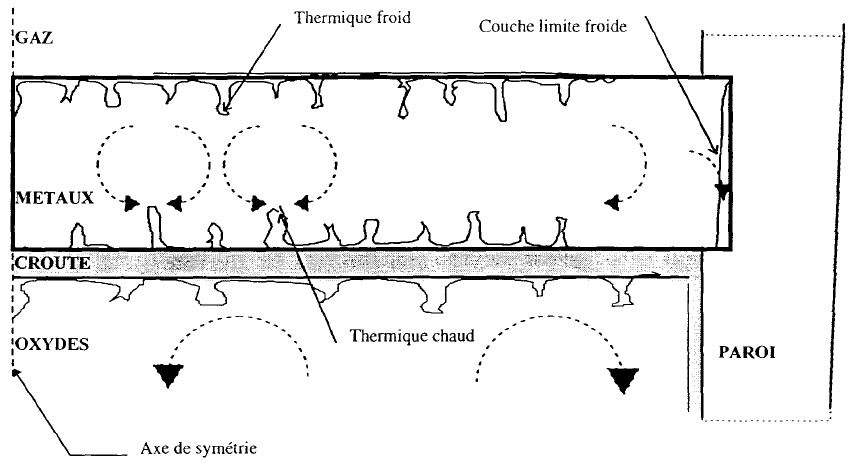
\includegraphics[width=0.8\textwidth]{Figures/metal_layer_flow.png}
    \end{column}
    \begin{column}{0.5\textwidth}
    \hskip -1cm \begin{minipage}{\textwidth}
    \begin{itemize}
    \item couche de fluide plus chaud en haut\\ $\rightarrow$ panaches (``thermiques'') chauds intermittents
    \item couche de fluide plus froid en haut \\ $\rightarrow$ panaches froids intermittents
    \item couche limite froide latérale \\ $\rightarrow$ accélération locale
    \end{itemize}
    \end{minipage}
    \end{column}
\end{columns}
\item Transition d'un écoulement laminaire à turbulent ``a partir'' de $H \sim10$cm
\item \emph{En première approche}, écoulement appréhendé comme la \emph{``juxtaposition''} de cellules de \emph{convection Rayleigh-Bénard} et d'une \emph{recirculation à la frontière latérale}
\end{itemize}
\end{frame}
\subsubsection{Conditions thermiques en limites axiales : instabilité de Rayleigh-Bénard}
\Titre{Couche métallique supérieure - instabilité de Rayleigh-Bénard}
\begin{frame}[fragile]
\begin{itemize}
\item Ecoulement \emph{conditionnellement instable} $Ra>Ra_c$ et transition \emph{laminaire - turbulent} (``douce'' puis ``dure'' puis ``asymptotique'')
\begin{minipage}{0.9\textwidth}
\begin{tabular}{cc}
\tiny{(Figures tirées de \cite{Gauthier2008})} & \multirow{2}{*}{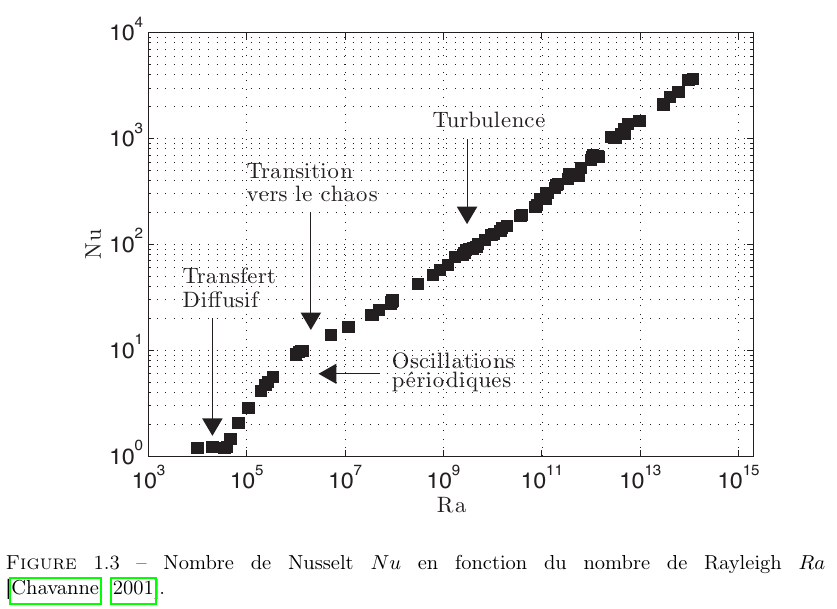
\includegraphics[width=0.5\textwidth]{Figures/Fig1_3_Gauthier2008.png}} \\
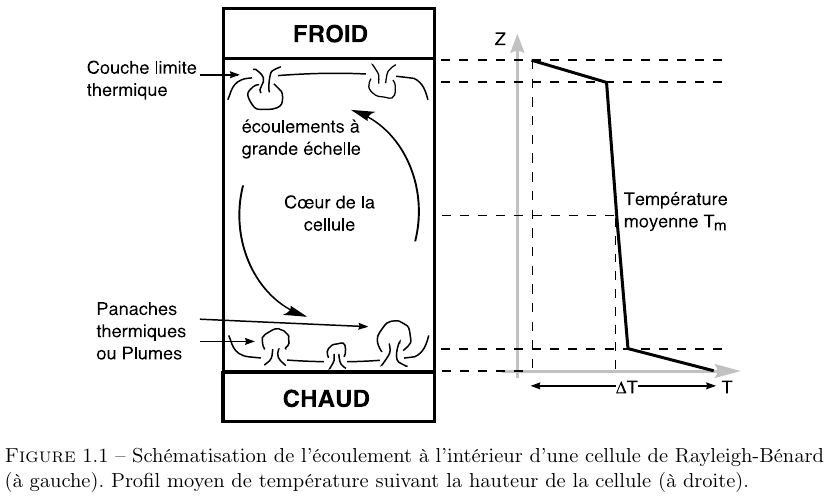
\includegraphics[width=0.5\textwidth]{Figures/Fig1_1_Gauthier2008.png} & \\
\end{tabular}
\end{minipage}
\vskip \baselineskip 
\item turbulence ``douce'' ($Ra_t<Ra<10^7$) : hypothèse de Markus (couches limites haute et basse indépendantes) $\rightarrow$ épaisseur $\delta = \frac{H}{2 Nu}$ indépendante de $H$ $\rightarrow$ $Nu \propto Ra^{\frac{1}{3}}$
\item au-delà, turbulence ``dure'' $\rightarrow$ $Nu \propto Ra^{\frac{2}{7}}$ ; asymptotique $\rightarrow$ $Nu \propto Ra^{\frac{1}{2}}$
\end{itemize}
\begin{tiny}
\begin{remark}[H. Bénard (1900)]
``Je n’ai pas la prétention d’avoir épuisé un sujet aussi nouveau : bien des points restent à éclaircir, même sans sortir du point de vue expérimental ; mais je serais heureux si mon travail, tout incomplet qu’il est, contribuait à attirer l’attention des expérimentateurs sur les domaines inexplorés de la Physique moléculaire et de la Mécanique des fluides''
\end{remark}
\end{tiny}
\vskip -0.5\baselineskip 
\scriptsize $\rightarrow$ Un v\oe u exaucé ! Toujours \emph{un sujet ``intense'' de recherche} (simulation numérique et expérience)
\end{frame}
\subsubsection{Conditions thermiques en limite latérale : refroidissement}
\Titre{Couche métallique supérieure - refroidissement latéral}
\begin{frame}[fragile]
\begin{itemize}
\item Ecoulement \emph{inconditionnellement instable} \begin{minipage}{0.05\textwidth}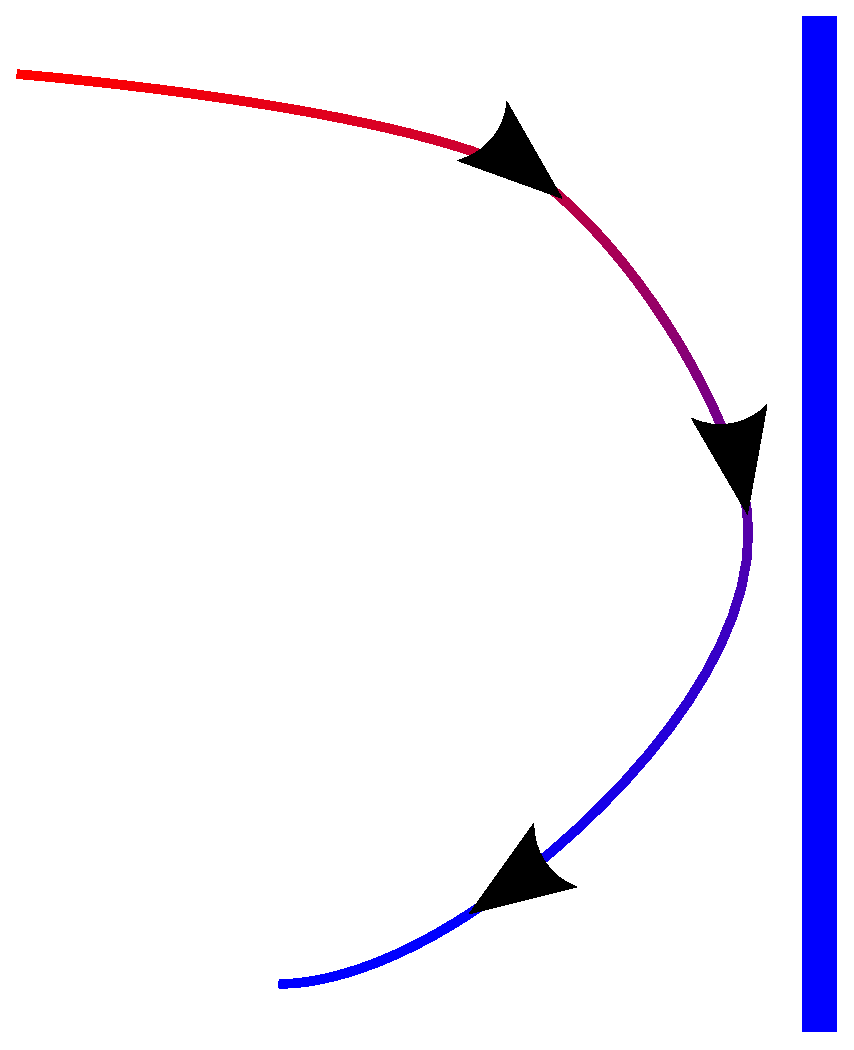
\includegraphics[width=\textwidth]{Figures/vertical_plate.eps} \end{minipage}
\item \emph{Impact sur le profil de température} pour $Pr$ faible {\tiny (Figure tirée de \cite{Tran2013})} \\
\begin{center} \vskip -\baselineskip ~ \\ 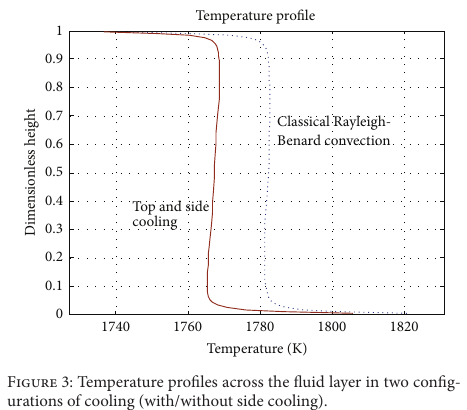
\includegraphics[width=0.4\textwidth]{Figures/Fig3_Tran2013.png} \end{center}
\item Malgré (à cause ?) de la complexité pour cette couche métallique, les \emph{modèles intégraux} ou ``grossièrement maillés'' ont recours à des \emph{corrélations} établies séparément pour des \emph{configurations ``unidimensionnelles''} $\rightarrow$ \textit{cf.} TD
\item Avec des limites (et des perspectives) que nous aborderons en 2$^{\text{ème}}$ partie de cours
\end{itemize}
\end{frame}

%%%%%%%%
\subsection{Thermohydraulique du bain oxyde}
\subsubsection{Solidification à l'interface}
\Titre{Bain oxyde - solidification à l'interface}
\begin{frame}[fragile]
\begin{columns}[T]
    \begin{column}{0.25\textwidth}
\centering 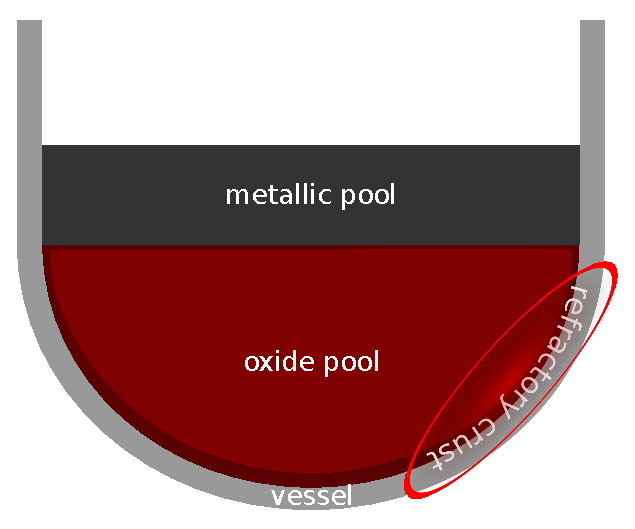
\includegraphics[height=0.3\textheight]{Figures/TD_2layer_crust.eps}
    \end{column}
    \begin{column}{0.75\textwidth}
\begin{itemize}
\item Corium oxyde : \emph{système ternaire} $\left(U_y,Zr_{1-y}\right)O_{2-x}$ ``en manque d'oxygène'' ($x\ge0$)
\item Température de liquidus $T_{liq}^{oxyde} \in [2300, 2950]$K suivant $y$ et $x$, toujours supérieur à $T_{liq}^{acier} \sim 1600$K $\rightarrow$ \emph{solidification à l'interface bain oxyde/cuve}
    \end{itemize}
    \end{column}
\end{columns}
\begin{minipage}{0.8\textwidth}
\begin{tabular}{cc}
\tiny{Figures tirées de \cite{Quaini2015} (échantillon $O_{0.39}U_{0.103}Zr_{0.507}$}) & \multirow{2}{*}{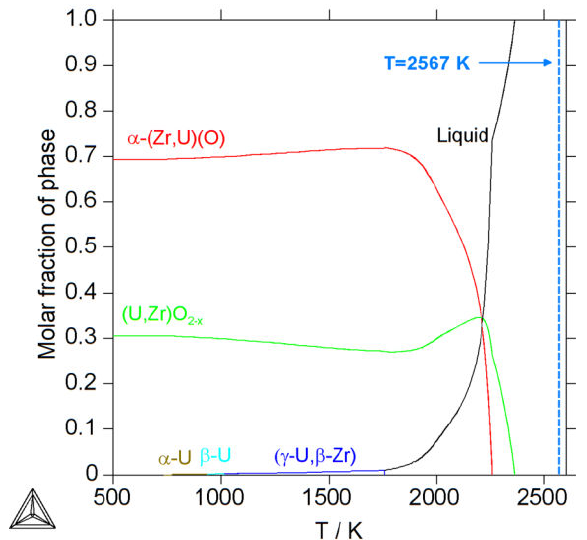
\includegraphics[width=0.42\textwidth]{Figures/Fig18a_Quaini2015.png}} \\
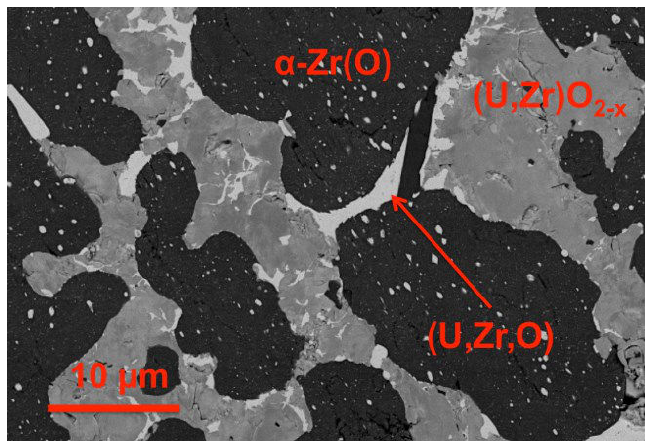
\includegraphics[width=0.5\textwidth]{Figures/Fig18b_Quaini2015.png} & \\
\tiny{microstructure observé} & \tiny{chemin de solidification (``lever-rule'') calculé}
\end{tabular}
\end{minipage}
\begin{itemize}
\item Solidification d'un \emph{matériau multicomposant} potentiellement \emph{compliquée} ... 
\end{itemize}
\end{frame}
\begin{frame}[fragile]
\begin{itemize}
\item ... corium $\left(U_y,Zr_{1-y}\right)O_{2-x}$ : le plus souvent, les \emph{hypothèses simplificatrices} suivantes :
\begin{itemize}
  \item un \emph{front de solidification à l'équilibre thermodynamique} $\rightarrow$ phase solide formée associée $\left(U_{y'},Zr_{1-y'}\right)O_{2-x'}$ à la température de liquidus du liquide à l'interface 
  \item \emph{variations de composition négligées} (liquide homogène et $x'=x$, $y'=y$)
\end{itemize}
\item Ainsi, \emph{comme pour un ``corps pur''}, solidification à l'interface régit par le déplacement d'un \emph{front plan} (\emph{condition de Stefan}, cas particulier du thèorème de Kotchine)
\begin{itemize}
  \item température imposée à l'interface $T^{\textrm{ls}}=T_{liq}^{oxyde}$
  \item condition de saut sur les flux à l'interface liquide/solide $\textrm{ls}$ : 
\begin{columns}
\begin{scriptsize}
\begin{column}{0.55\textwidth}
\begin{eqnarray*}
  \vec{v}^{\textrm{ls}}(\vec{r}, t) &=& \frac{\vec{n}^{\textrm{ls}}}{\rho_l \Delta h_{ls}} \left(-\lambda_l \grad{T_l}(\vec{r}, t) + \lambda_s \grad{T_l}(\vec{r}, t) \right) \cdot \vec{n}^{\textrm{ls}} \\
  &&\text{(vitesse locale)}\\
  \frac{dm^{\textrm{ls}}(t)}{dt} &=& \frac{1}{\Delta h_{ls}} \left(\phi_l^{\textrm{ls}}(t) - \phi_s^{\textrm{ls}}(t)\right) S^{\textrm{ls}} \\
  && \text{(débit massique intégral)}
\end{eqnarray*}
\end{column}
\begin{column}{0.45\textwidth}
\begin{itemize}
\item $\vec{n}^{\textrm{ls}}$ : normal orientée du liquide vers le solide
\item $\Delta h_{ls}$ : chaleur latente spécifique de solidification
\end{itemize}
\end{column}
\end{scriptsize}
\end{columns}
\end{itemize}
\item En géométrie \emph{1D plan}, en  \emph{régime stationnaire}, épaisseur du solide (sans dissipation interne de puissance) donnée par \emph{$e_{s} = \lambda_{s}\times \frac{\text{différence de température d'un bord à l'autre}}{\text{flux de chaleur}}$}
\end{itemize}
\end{frame}
\subsubsection{Convection naturelle par chauffage volumique}
\Titre{Bain oxyde - convection naturelle par chauffage volumique}
\begin{frame}[fragile]
\begin{columns}[T]
    \begin{column}{0.25\textwidth}
\centering 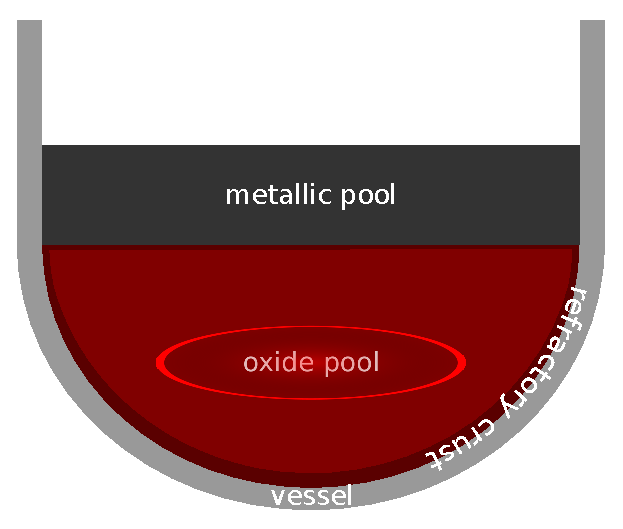
\includegraphics[height=0.3\textheight]{Figures/TD_2layer_oxide.eps}
    \end{column}
    \begin{column}{0.75\textwidth}
\begin{itemize}
    \item \emph{chauffage ``en volume''} (puissance résiduelle associée à la décroissance des produits de fission) : puissance volumique $q^{ox}$ (W/m$^3$)
    \item refroidissement en surfaces latérale et haute
    \item en \emph{régime turbulent} : $Ra_i^{ox}=\frac{g\left(H^{ox}\right)^5q^{ox}\beta^{ox}}{\lambda^{ox}\nu^{ox}\alpha^{ox}} \in [10^{14}, 10^{18}]$
    \end{itemize}
    \end{column}
\end{columns}
\begin{itemize}
\item Schéma de l'écoulement (Figure tirée de \cite{Bonnet1999})
\begin{columns}[T]
    \begin{column}{0.6\textwidth}
\centering 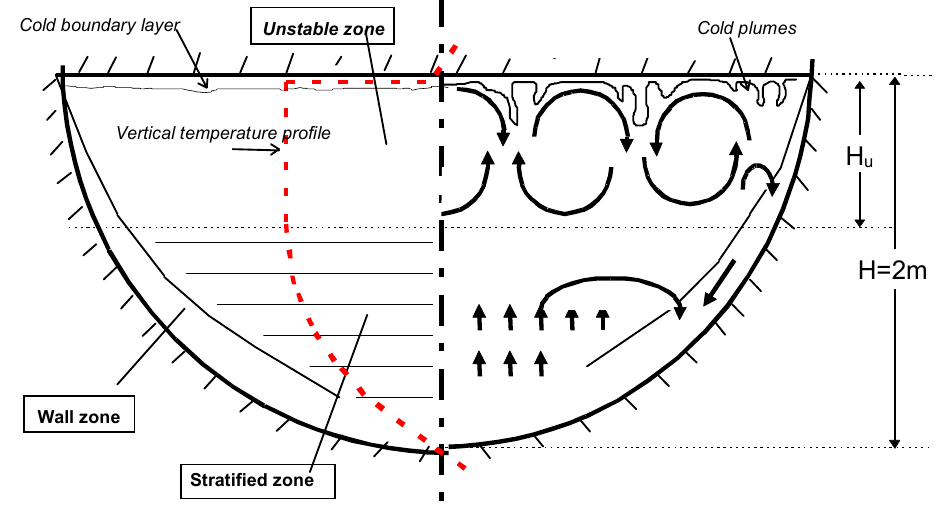
\includegraphics[width=0.8\textwidth]{Figures/Fig2_Bonnet2001.png}
    \end{column}
    \begin{column}{0.5\textwidth}
    \hskip -1cm \begin{minipage}{\textwidth}
    \begin{itemize}
    \item panaches froids et boucles de convection en haut
    \item couche limite froide latérale
    \item zone stratifiée thermiquement en bas
    \end{itemize}
    \end{minipage}
    \end{column}
\end{columns}
\end{itemize}
\end{frame}
\begin{frame}[fragile]
\begin{itemize}
\item En première approche, pour l'\emph{échange vers le haut}, parallèle entre cette \emph{configuration de ``Kulacki-Emara''} et une \emph{cavité de Rayleigh-Bénard} de hauteur $H_u$
\begin{columns}[T]
    \begin{column}{0.25\textwidth}
\centering 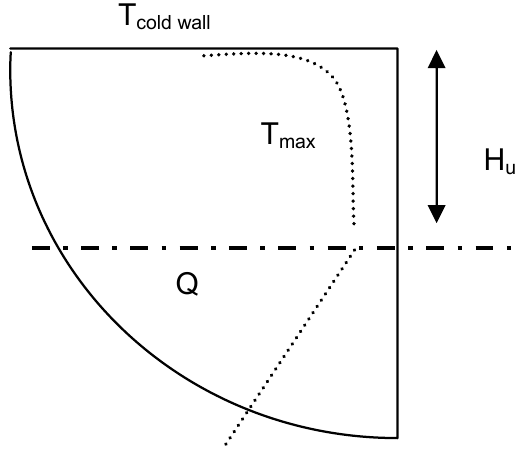
\includegraphics[width=1.0\textwidth]{Figures/p11_1_Bonnet2001.png}
    \end{column}
    \begin{column}{0.5\textwidth}
\centering 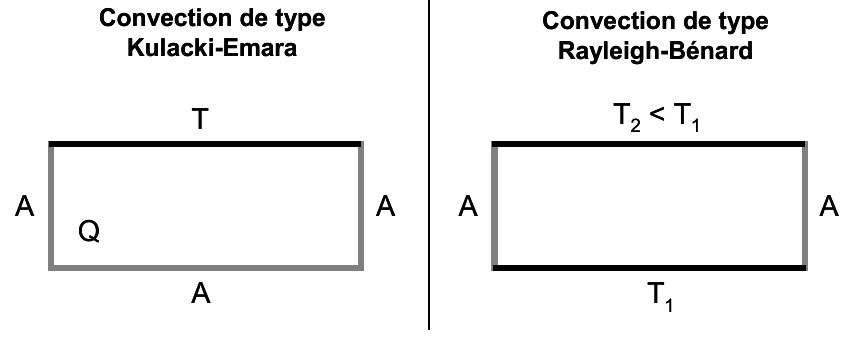
\includegraphics[width=1.0\textwidth]{Figures/KE_RB.png}
    \end{column}
    \begin{column}{0.25\textwidth}
\centering 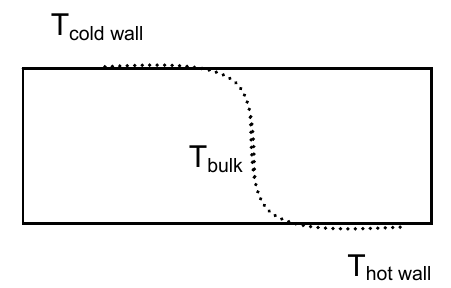
\includegraphics[width=1.0\textwidth]{Figures/p11_2_Bonnet2001.png} 
    \end{column}
\end{columns}
\begin{itemize}
  \item avec un nombre de Rayleigh exprimé en fonction de $\Delta T = \left(T_{max}-T_{cold\, wall}\right)$ et $H_u$
  \item à l'état stationnaire : $S_{up} \times \left(\frac{\lambda Nu_{up}}{H_u}\right) \Delta T = V \times q$
  \item ainsi, on peut travailler en nombre de \emph{Rayleigh interne} $Ra_i=\frac{g\left(H_u\right)^5\emph{q}\beta}{\lambda\nu\alpha}$ : \\
  $Nu^{RB}_{up} = a \times Ra^b Pr^c \Longleftrightarrow Nu^{KE}_{up} = 2a^{\frac{1}{b+1}} \times Ra_i^{\frac{b}{b+1}} Pr^{\frac{c}{b+1}}$
\end{itemize}
\item Pour l'\emph{échange latéral} (surface sphéro\"{\i}de), la \emph{transposition est moins évidente} ...
\end{itemize}
\end{frame}
\begin{frame}[fragile]
\begin{itemize}
\item ... de nombreuses \emph{expériences} ont été menées sur des  \emph{``géometries fond de cuve''} à échelle réduite avec différents matériaux simulants
\begin{columns}[T]
    \begin{column}{0.72\textwidth}
      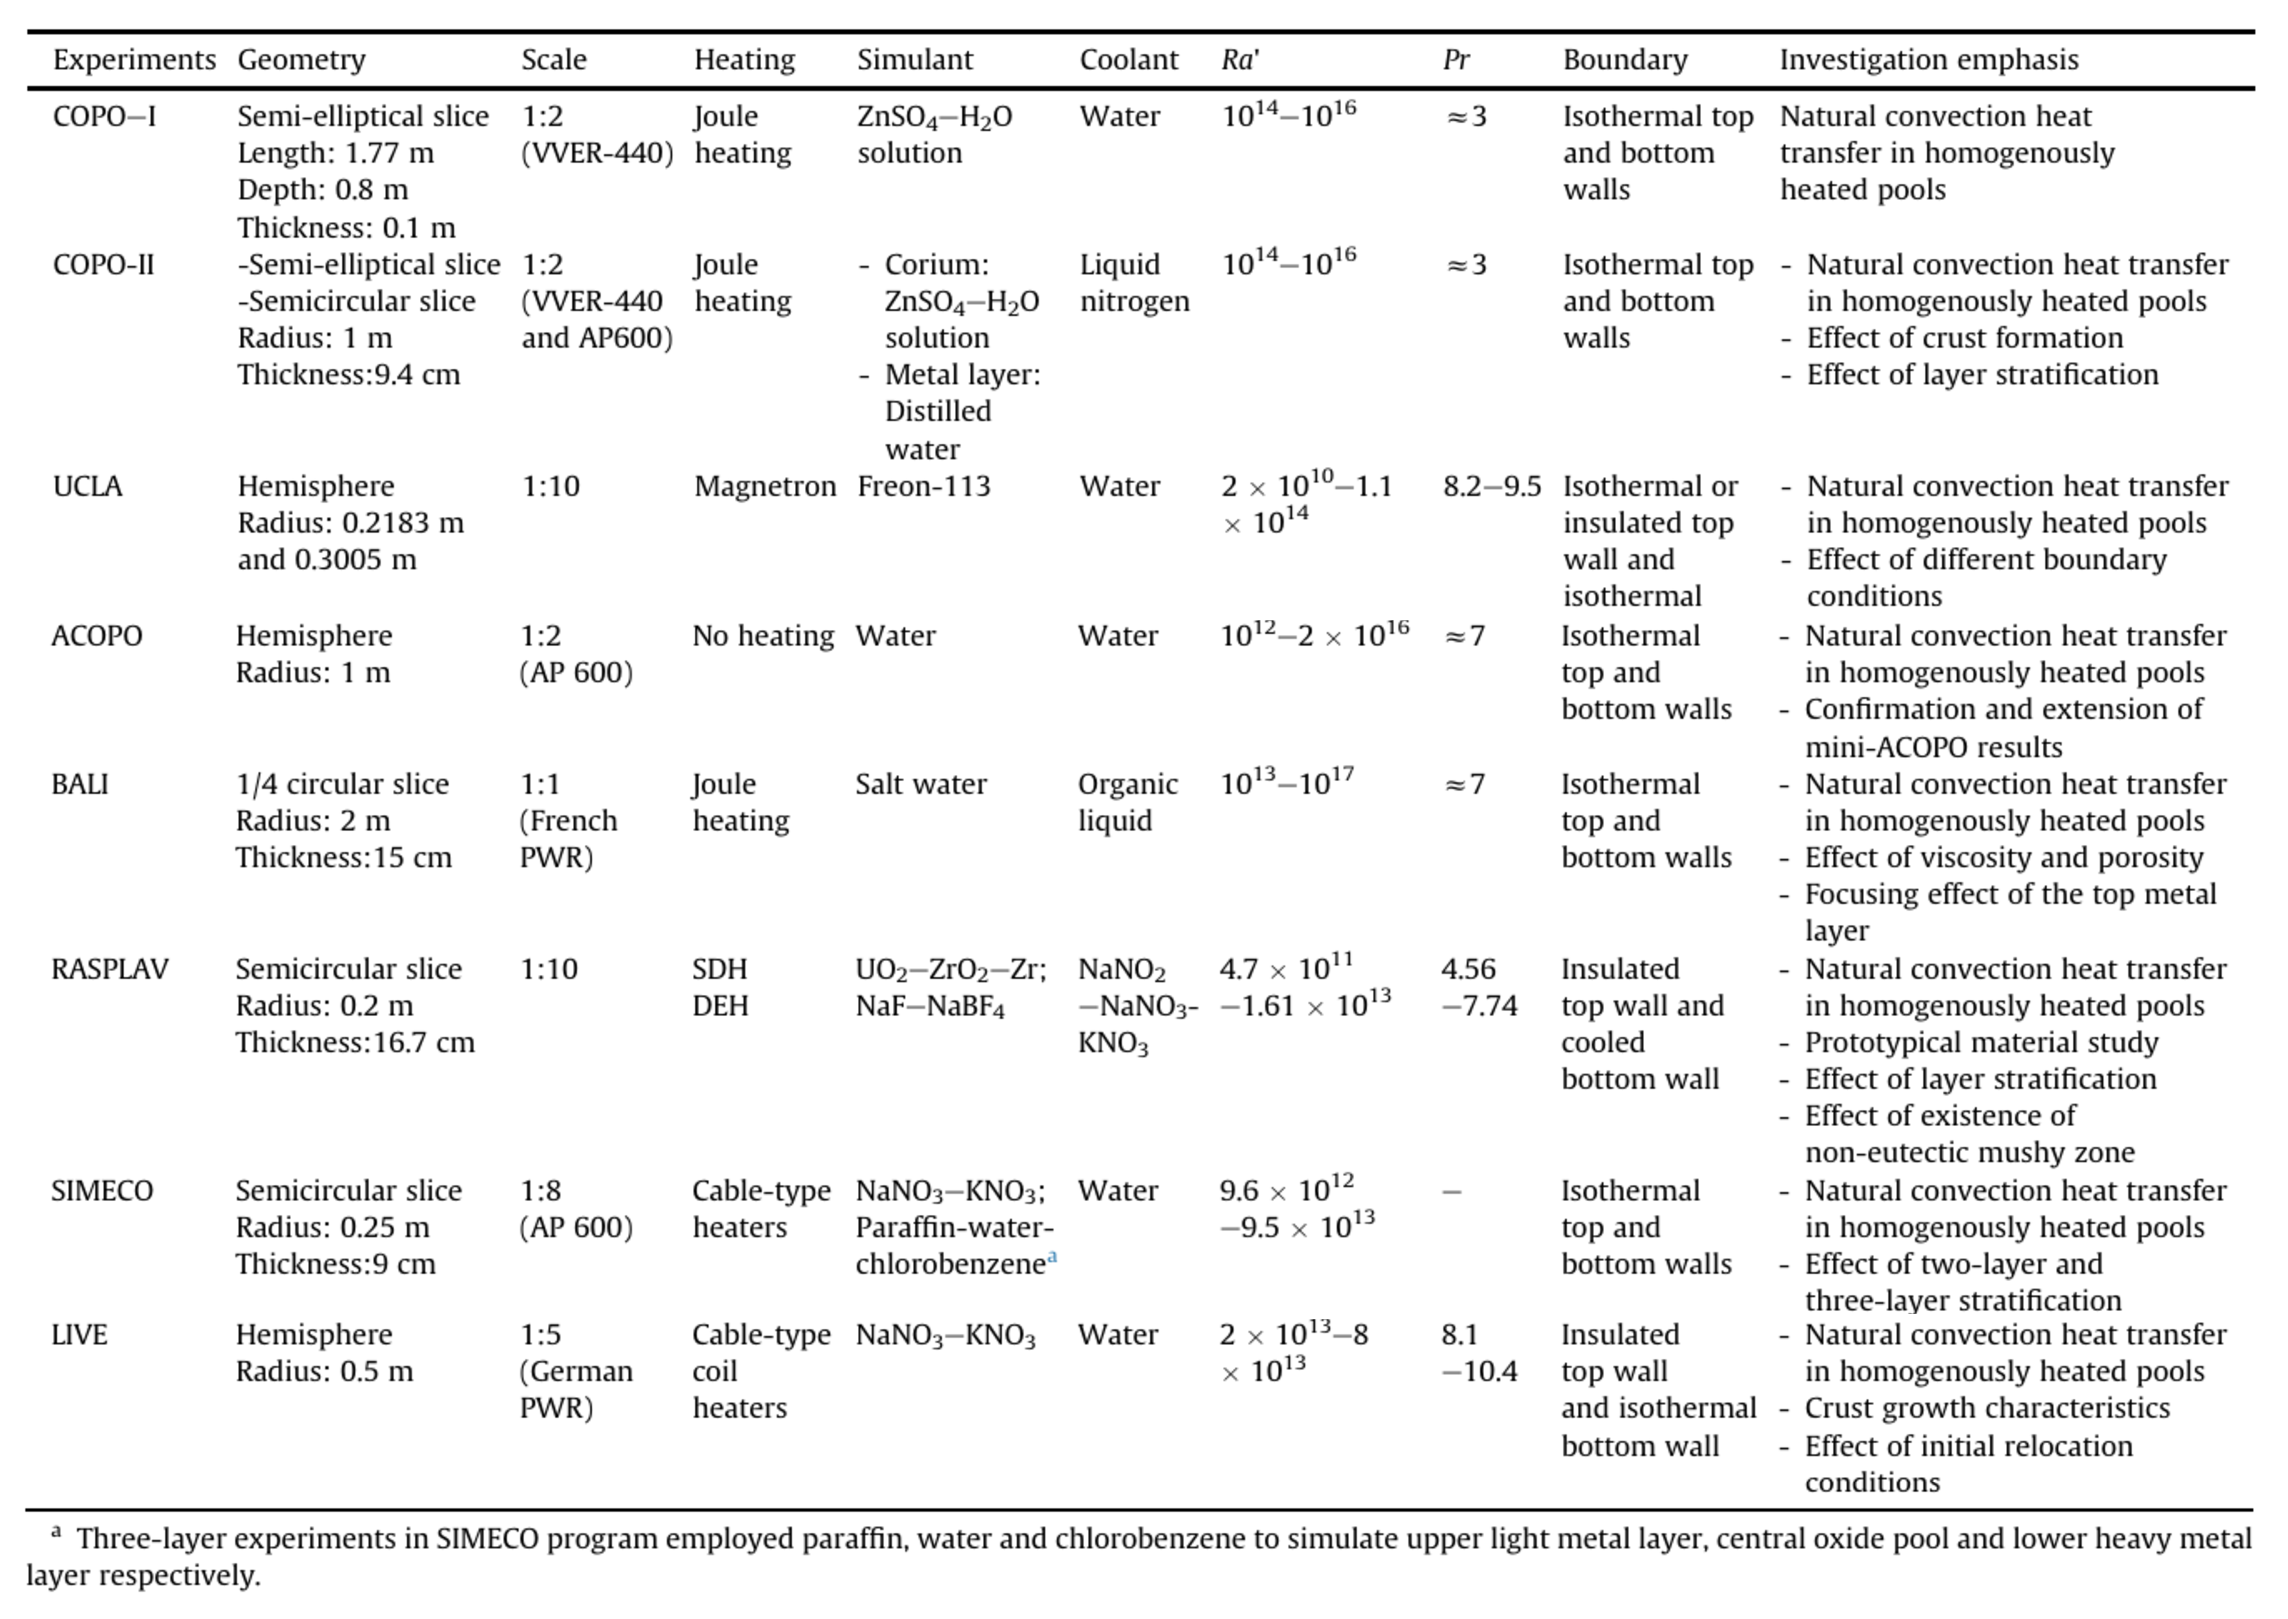
\includegraphics[height=0.8\textheight]{Figures/Tab3_Zhang2015.eps} \\
      {\tiny extrait d'un tableau de \cite{Zhang2015}}
    \end{column}
    \begin{column}{0.28\textwidth}
    \vskip -\baselineskip
    \centering
{\tiny BALI} \\ 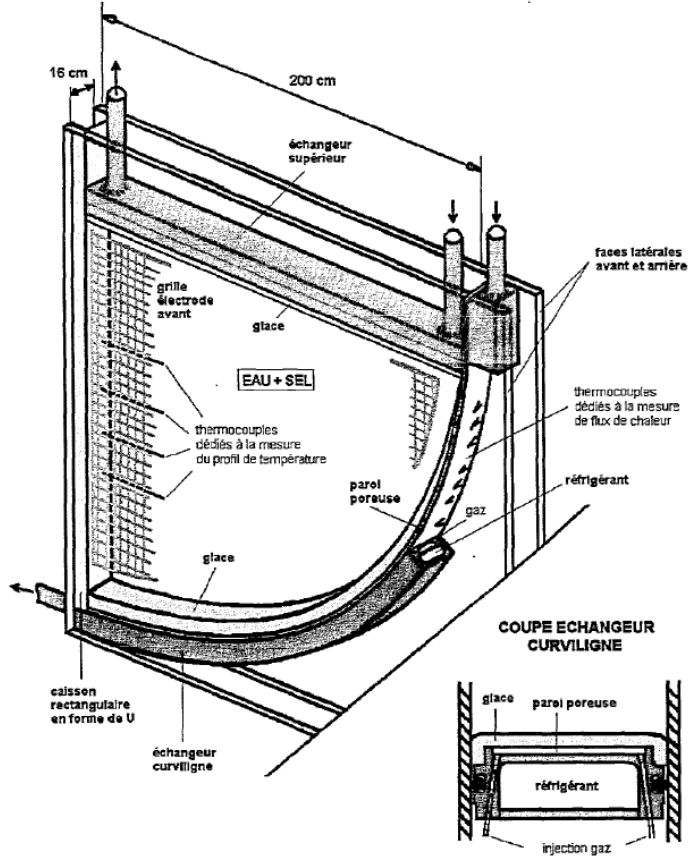
\includegraphics[width=1.0\textwidth]{Figures/bali.png} \\ 
{\tiny LIVE} \\ 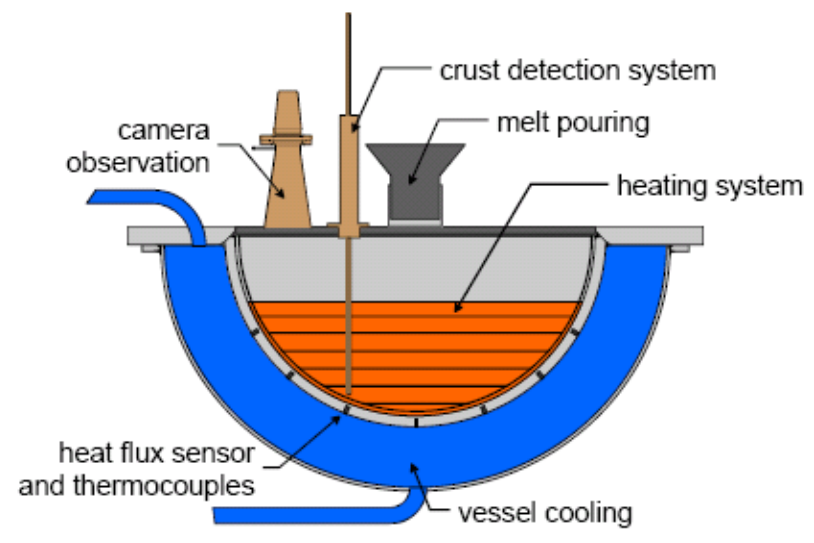
\includegraphics[width=1.0\textwidth]{Figures/live_1.png}
% 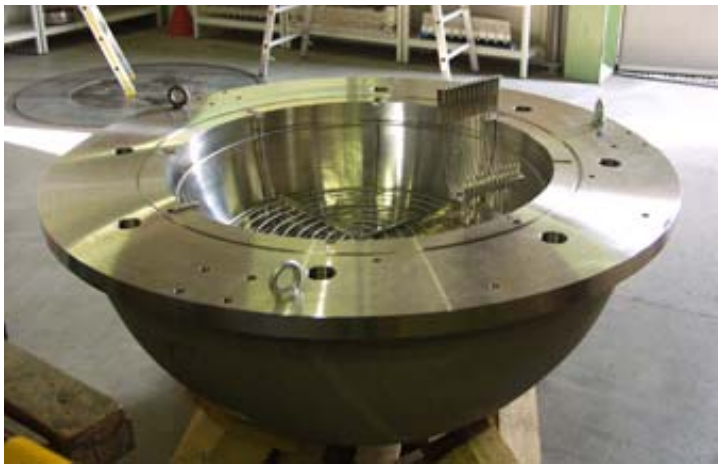
\includegraphics[width=1.0\textwidth]{Figures/live_2.png}
    \end{column}
\end{columns}
\end{itemize}
\end{frame}
\begin{frame}[fragile]
\begin{itemize}
\item Qui fournissent des \emph{corrélations} pour fermer les bilans des \emph{modèles intégraux}
\item Une \emph{dispersion des résultats qui augmente avec $Ra_i$} \danger
\begin{columns}[T]
    \begin{column}{0.4\textwidth}
\centering 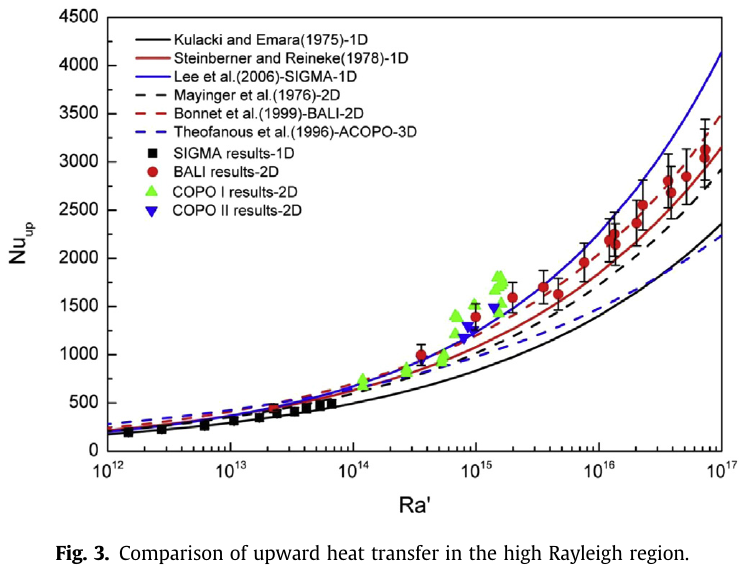
\includegraphics[width=1.0\textwidth]{Figures/Fig3_Zhang2015.png}
    \end{column}
    \begin{column}{0.4\textwidth}
\centering 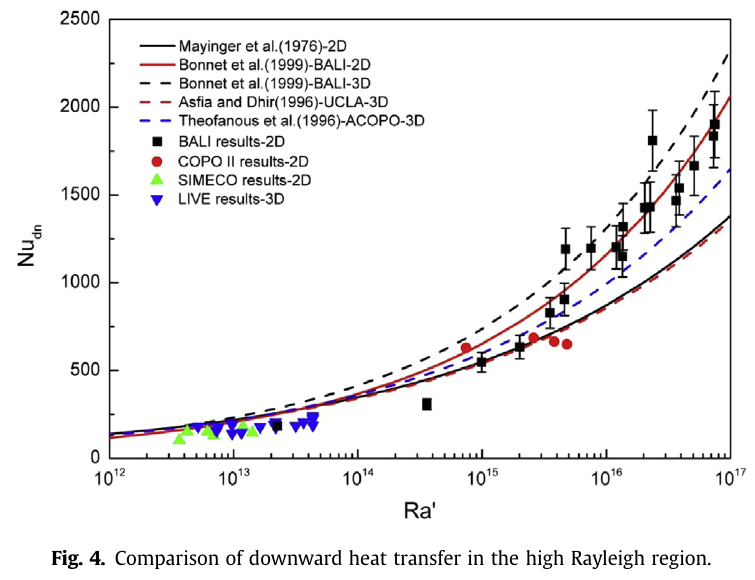
\includegraphics[width=1.0\textwidth]{Figures/Fig4_Zhang2015.png}
    \end{column}
\end{columns}
{\tiny (Figures tirées de \cite{Zhang2015})}
% \item ... mais pas une source majeure d'incertitude pour l'évaluation de l'IVR
\end{itemize}
\vskip -\baselineskip
\begin{columns}[T]
    \begin{column}{0.4\textwidth}
\begin{itemize}
\item Intérêt grandissant pour des simulations ``Computational Fluid Dynamics'' CFD
\end{itemize}
    \end{column}
    \begin{column}{0.6\textwidth}
\vskip -0.5\baselineskip
\centering 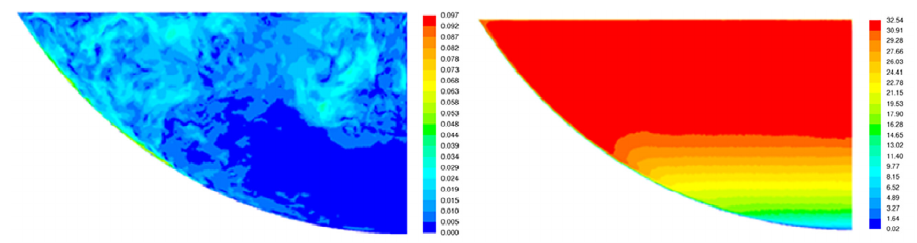
\includegraphics[width=1.0\textwidth]{Figures/Fig10a_Shams2019.png} \\ 
\vskip -0.5\baselineskip
{\tiny vitesse et température - calcul CFD-LES - essai BALI 1-15}
    \end{column}
\end{columns}
\vskip -\baselineskip
\centering {\tiny (Figure extraite de \cite{Shams2020})}
\end{frame}
%%%%%%%%
\subsection{TD : évaluation du bilan thermique intégral}
\Intercalaire{TD : évaluation du bilan thermique intégral}
\Titre{TD : évaluation du bilan thermique intégral}
\begin{frame}[fragile]
\begin{columns}[T]
    \begin{column}{0.4\textwidth}
      \begin{figure}[H]
\centering 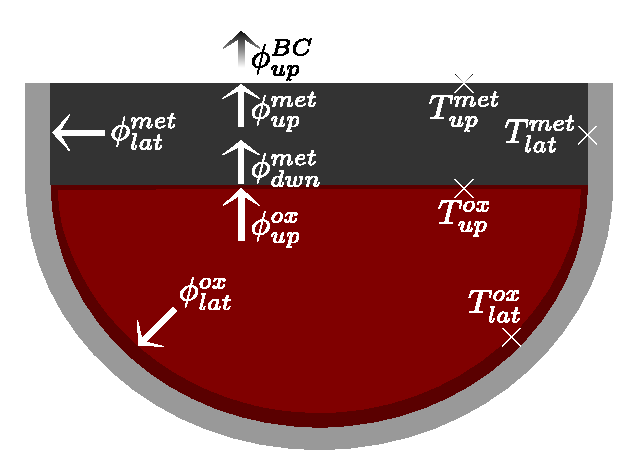
\includegraphics[height=0.4\textheight]{Figures/TD_2layer.eps}
\caption{Configuration à deux couches et notations des flux et températures}
      \end{figure}
    \end{column}
    \begin{column}{0.6\textwidth}
    \begin{itemize}
    \item Objectif: évaluation de la \emph{répartition de la puissance et du flux de chaleur} aux interfaces d'un bain de corium
    \item \emph{Configuration stationnaire à deux couches} :
    \begin{itemize} 
    \item en bas : une phase oxyde qui porte toute la puissance résiduelle entourée d'une croûte réfractaire 
    \item en haut : de l'acier liquide en contact direct avec la paroi de la cuve en fusion
    \end{itemize}
    \item Hypothèses et fermetures classiquement utilisées dans les codes de calculs (et que l'on vient de présenter pour la plupart)
    \end{itemize}
    \end{column}
\end{columns}
\vskip \baselineskip
\textit{cf.} description TD et notebooks Jupyter %\\ {\scriptsize (\href{https://mybinder.org/v2/gh/niamorelreillet/ENSE3---TD/master?urlpath=lab}{https://mybinder.org/v2/gh/niamorelreillet/ENSE3---TD/master?urlpath=lab})}
\end{frame}